\documentclass[tikz,border=1mm,10pt]{standalone}
%\usepackage[dvipsnames]{xcolor}
\usepackage{pgfplots}
\pgfplotsset{compat=1.5.1}
\begin{document}
	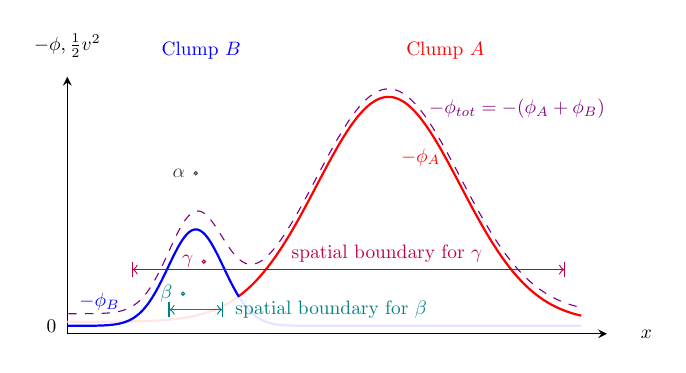
\begin{tikzpicture}[xscale=1,yscale=1,samples=400, transform shape,every node/.style={scale=0.7}]
	\begin{axis}[
	ticks=none,
	ymin=0,
	ymax=16,
	xmin=-8,
	xmax=25.6,
	axis x line=bottom,axis y line=left,
	%	axis lines = left,
	xlabel = $x$,
	ylabel = {$- \phi, \frac{1}{2}v^2$},
	legend pos=north west,
	every axis x label/.style={
		at={(ticklabel* cs:1.05)},
		anchor=west,
	},
	every axis y label/.style={
		at={(ticklabel* cs:1.05)},
		anchor=south,
	},
	axis equal image
	]
	
	%clump A
	\addplot [
	domain=2.66584:24, 
	samples=400, 
	color=red,thick
	]
	{14*exp(-(x-12)^2/40)+0.75};
	\addplot [
	domain=-10:2.66584, 
	samples=400, 
	color=red!10,thick
	]
	{14*exp(-(x-12)^2/40)+0.75};

	%clump B
	\addplot [
	domain=2.66584:24, 
	samples=400, 
	color=blue!10, thick
	]
	{6*exp( (-x^2)/6)+0.5};
	\addplot [
	domain=-10:2.69, 
	samples=400, 
	color=blue, thick
	]
	{6*exp( (-x^2)/6)+0.5};
	
	%totalplot
	\addplot [
	domain=-10:24, 
	samples=400, 
	color=violet,
	style=dashed
	]{6*exp( (-x^2)/6)+0.5 + 14*exp(-(x-12)^2/40)+0.75};
%	\addlegendentry{$\phi_A+\phi_B$}
	%
	%
	
	% Particles
	\draw[darkgray] (100,100) circle (.1) node [left = .7mm] {$\alpha$};
	%\draw[cyan] (110,70) circle (.1) node [right = .7mm] {$\beta$};
	\draw[purple] (105,45) circle (.1) node [left = .7mm] {$\gamma$};
	\draw[teal] (92,25) circle (.1) node [left = .7mm] {$\beta$};
	\draw[|<->|, color=purple] (60,40) -- node [right = 7mm, above=.1mm] {spatial boundary for $\gamma$} (330,40) ;
	\draw[|<->|,color=teal] (83,15) -- (117,15) node [right=1mm] {spatial boundary for $\beta$};
	%
	%
	%Naming
	\node[thick, blue] at (40,20) {$-\phi_B$};
	\node[thick, red] at (240,110) {$-\phi_A$};
	\node[thick, violet] at (300,140) {$-\phi_{tot}=-(\phi_A+\phi_B)$};
%	\draw[color=black,style=dashed] (100+26.6584,25) -- (100+26.6584,120) node [above=1mm] {saddle};
	
	
	\end{axis};
	\node[] at (-0.2,0.1) {$0$};
	\node[thick, blue] at (1.7,3.6) {Clump $B$};
	\node[thick, red] at (4.8,3.6) {Clump $A$};
	\end{tikzpicture}
\end{document}